\chapter{Tool Development}
This chapter focuses on the development of two essential tools designed to streamline the process of creating and evaluating blockchain protocols, particularly on the Tezos platform. The first tool, known as the Bootstrapper, automates the initial setup and coding tasks, providing a quick start for developers. The second tool, the Live Testing Tool, offers a real-world testing environment equipped with a variety of features for performance metrics and network control. Together, these tools aim to address the complexities and challenges inherent in blockchain protocol development, offering a more accessible and efficient pathway for both novice and experienced developers.


\section{Bootstrapping Tool}
The Bootstrapper was conceived with the aim of simplifying the development process for creating new protocols in Tezos. Our objective was to minimize the amount of code a developer needs to write to get a protocol up and running. To achieve this, we carefully selected code components that are generic enough to be applicable across multiple protocols. Additionally, we automated certain aspects of the protocol's integration with both Tezos and our Testing tool. In essence, the Bootstrapper serves as a scaffolder or starter pack for protocol development in Tezos.

\subsection*{Protocol Generalizations and Common Code}

As previously mentioned in the document, there are specific requirements that every protocol must meet to be compatible with Tezos:

\begin{itemize}
\item Must reside in the `src` folder within the Tezos codebase.
\item Must contain a `lib\_protocol` folder and a `main.ml` file.
\item Requires a `dune` file, as Tezos utilizes the Dune build system.
\item Must include a `TEZOS\_PROTOCOL` JSON file with attributes:
\begin{itemize}
  \item `expected\_env\_version`: Expected environment version. Defaults to version 6 for simplicity but can be changed.
  \item `hash`: Protocol's hash, serving as its identifier within the node.
  \item `modules`: Names of the OCaml Modules within the folder.
\end{itemize}

\end{itemize}

Our tool automates the creation of these required components, eliminating the need for manual setup.

\subsubsection*{Common Code Components}

Here we outline the elements that are common across most protocols.

\textbf{Main.ml File}: Since we use environment v6, a `main.ml` file is included with the essential layout. This is one of the few components that can't be generalized, as it contains the protocol's logic.
  
\textbf{Account and Tez Representation}: Most protocols have the concept of users/accounts and balances. Therefore, we include representations for accounts and Tez, the currency in this system.

\textbf{Storage Logic, Functors, and More}: We include abstractions for storage in Tezos, utilizing the concept of Maps for key-value storage, which is common to most protocols.

\textbf{Block Header Representation}: Every protocol needs to define how it will represent the header part of its blockchain. This is a common requirement, although the specific characteristics may vary.

Given these commonalities, our tool serves as a starter kit, providing the essential components that can be generalized across different protocols. The tool aims to fill in as much as possible, leaving only the unique logic to be implemented by the developer.


\subsubsection*{Functionalities}
The Bootstrapper is a command-line program designed to streamline the initial setup of a new protocol in Tezos.
It functions as an "Init Protocol" command, performing the following tasks of \textbf{folder creation}, where it automatically sets up the necessary folders, \textbf{template copy}, as it copies a predefined template (created by us) into the new folder, but are left in the folder so the developer can change it for their needs, \textbf{text replacement and integration}, as it replaces specific text in the template and ensures integration with Tezos' Dune build system and other required code components, and finally it \textbf{includes a pre built script} to build the protocol, so there's no need for the developer to learn how this process is done.

To further ease development and reduce boilerplate code, we enhanced a pre-existing meta-programming library, \textit{ppx\_deriving\_encoding} ADICIONAR REFERENCIA. 
This library allows developers to automate the definition of encoding functions, by appending a meta-programming tag \textit{[@@deriving encoding]} to a type, the encoding function for that type is automatically generated, and this is particularly useful for type representations, as a big part of the code in protocols are these functions.
We also include a block header functor, that auto-generates the entire block\_header file functionality by merely providing a type.
This not only reduces the code volume by threefold (as experienced while improving the previously mentioned Proof of Work) but also alleviates the developer's need to delve into the intricacies of the Data-encoding library.

For the user, this is abstracted with the following command

\textit{./bootstrapper -name my\_really\_fast\_protocol -env 6}





By incorporating these functionalities, the Bootstrapper serves as a comprehensive tool for initiating and easing the development of new protocols in Tezos.





\section{Live Testing Tool}

The Live Testing Tool is central to the main objective of this thesis, which aims to facilitate the development and evaluation of blockchain protocols in a live setting. After developing a protocol in a standardized manner, particularly using Tezos as the platform, the next crucial step is to observe its real-world behavior. This tool is designed to not only run the protocol in a live environment but also to provide valuable metrics about the network's performance. Additionally, it offers the capability to control various aspects of the network, allowing for a comprehensive evaluation of the protocol under different conditions, and can also be used during the development of the protocol as part of the development workflow, as with it it's possible to write tests and get a network running in way fewer steps as with manually executing commands and operations.

Overall, the Live Testing Tool serves as an essential component for both the development and assessment phases of blockchain protocols.



\subsection*{Functionalities}
The Live Testing Tool operates as a web server, making it language-agnostic for test development. Any programming language capable of making HTTP requests can interact with it. The server exposes a variety of endpoints that facilitate different aspects of testing, such as initiating a protocol test, controlling node operations, and gathering network metrics.

In its architecture, the server acts as a coordinator, maintaining a list of all node endpoints and ensuring seamless interaction among them. This enables the tool to have a centralized point for controlling and monitoring the network.

While it's executing, the tool also logs information about the tests it performed, from the protocols, to the start time of the nodes and more.

To provide real-time metrics and insights, the tool employs a monitoring mechanism for each node. Referred to as "watchers," these components continually request information from their respective nodes, focusing on blocks and transactions. This allows the tool to perform various calculations and assessments, offering a comprehensive view of the protocol's behavior in a live setting.


\begin{figure}[H]
    \centering
    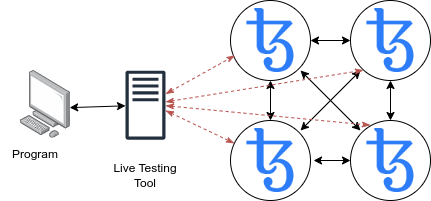
\includegraphics[width=\textwidth,keepaspectratio]{imagens/live_testing_tool.png}
    \caption{Live Testing Tool Architecture Visualized, with 4 Tezos Nodes Running}
    \label{fig:theorems}

\end{figure}



\subsection*{\textbf{Endpoints Provided by the Tool}}

\textbf{Generic Endpoints}
\begin{itemize}
  \item \texttt{/start-test}: Initiates a test network given the \textit{protocol name}, \textit{number of nodes}, and \textit{initial parameters}.
  \item \texttt{/stop-test}: Halts all ongoing tests and activities.
  \item \texttt{/status}: Displays the current status of the test.
  \item \texttt{/protocols}: Lists the protocols that the tool has detected.
  \item \texttt{/protocol-parameters/:name}: Retrieves the parameters of a specific protocol.
  \item \texttt{/nodes}: Returns information about each node, including \textit{IP}, \textit{ports}, \textit{process ID}, and \textit{directory}.
\end{itemize}

\textbf{Protocol-Related Endpoints}
\begin{itemize}
  \item \texttt{/swap-protocol}: Replaces the current protocol with another.
  \item \texttt{/change-parameters}: Alters the existing parameters of the network's protocol.
\end{itemize}

\textbf{Network Control Endpoints}
\begin{itemize}
  \item \texttt{/start-node/:id}: Starts a node with a specific \textit{ID}, if provided.
  \item \texttt{/stop-node/:id}: Stops a node with a specific \textit{ID}.
\end{itemize}

\textbf{Split Brain/Fork-Related Endpoints}
\begin{itemize}
  \item \texttt{/split-network}: Splits the network into smaller networks, given a list of nodes.
  \item \texttt{/rejoin-network}: Rejoins the fragmented networks into a single network.
\end{itemize}

\textbf{Metrics Endpoints}
\begin{itemize}
  \item \texttt{/tps}: Provides the max, min, and average \textit{Transactions Per Second}.
  \item \texttt{/time-to-consensus}: Measures the time taken for the majority of the network to agree on a block.
  \item \texttt{/propagation-times}: Calculates the time for a block to propagate across the network.
  \item \texttt{/first-and-last-block-times}: Gives the time of the first and last blocks.
  \item \texttt{/blocks-per-second}: Offers the max, min, and average blocks per second.
  \item \texttt{/discarded-blocks}: Indicates the number of blocks discarded by the network.
\end{itemize}


\subsection*{Example Usage}

In this section we showcase how this tool can be used from a Python script.

\begin{listing}[H]
\caption{Example function that starts a test}
\label{lst:python_code}
\begin{minted}[fontsize=\footnotesize]{python}
def start_test(protocol_name, nodes, fitness, parameters):
    data = {
        "protocol_name": protocol_name,
        "n_nodes": int(nodes),
        "fitness": int(fitness),
        "parameters": parameters
    }
    print(data)
    response = requests.post(ADDRESS + "/start-test", json=data)
    if response.status_code == 200:
        print("Success:", response.text)
    else:
        print("Failure:", response.status_code)
        exit(1)
\end{minted}
\end{listing}

\begin{listing}[H]
\caption{Multiple utility functions to fetch information about the network}
\label{lst:python_code}
\begin{minted}[fontsize=\footnotesize]{python}
# Function that returns the current status of the network
def get_status():
    return requests.get(ADDRESS + "/status").json()
# Function that returns information about all nodes
def get_nodes():
    return requests.get(ADDRESS + "/nodes").json()
# Function that returns the hash of the current head
def get_head_hash(node_rpc):
    return requests.get(f"http://127.0.0.1:{node_rpc}/chains/main/blocks").json()[0][0]
# Function that returns the info of a specific block, provided a hash (block_id)
def get_block_info(node_rpc, block_id):
    return requests.get(f"http://127.0.0.1:{node_rpc}/chains/main/blocks/{block_id}").json()
# Function that returns the info of the head
def get_head_info(node_rpc):
    return get_block_info(node_rpc, get_head_hash(node_rpc))
\end{minted}
\end{listing}




\begin{listing}[H]
\caption{Functions that request information in a loop}
\label{lst:python_code}
\begin{minted}[fontsize=\footnotesize]{python}
# Loop that keeps requesting the latest info about the tps of the system
async def fetch_tps():
    while True:
        async with requests.get(ADDRESS + "/tps") as response:
            tps = await response.text()
            print(f"Current TPS: {tps}")
        await asyncio.sleep(1)
# Loop that waits until the test is running
async def wait_for_start():
    last_status = 'stopped'
    while last_status != 'running':
        status_resp = get_status()
        last_status = status_resp["status"]
        sleep(1)
    return
\end{minted}
\end{listing}

\begin{listing}[H]
\caption{Main Function that tests how the TPS changes with the Block Time}
\label{lst:python_code}
\begin{minted}[fontsize=\footnotesize]{python}
# Main function that preforms the test
# In this test we check out what happens to TPS when we duplicate the Block Time
def test():
    blocks_to_wait = 200 # Blocks to wait until we increase the Block Time
    protocol_name = "demo" # Name of the protocol
    current_block_time = 60 # In seconds
    parameters = get_protocol_parameters(protocol_name) # Fetch parameters 
    number_of_nodes = 20 # Number of nodes to start the network
    fitness = 0 
    # we change the default parameters so it has the block time specified
    parameters["constants"]["block_time"] = current_block_time

    # We start the test and wait until the network is ready
    start_test(protocol_name, number_of_nodes, 0, parameters)
    wait_for_start()

    # Ommited function, that fetches information about the nodes
    nodes = get_nodes()
    first_node = nodes[0] 

    # Ommited function that makes it so the first node has an baker executing
    # MINER_ADD is the address of the miner
    start_mine(first_node, MINER_ADD)

    # Ommited function that spams the network with transactions
    spam_transactions(nodes, MINER_ADD)

    # We show the current TPS in the command line
    fetch_tps()

    while True:
        last_block_info = get_head_info(first_node)
        level = last_block_info["header"]["level"]
        
        # In case we reached the level of blocks to wait, we increase the block_time
        if level % blocks_to_wait == 0:

            current_block_time = current_block_time * 2
            parameters["constants"]["block_time"] = current_block_time

            print("Increasing the Block Time to " + current_block_time)
            change_parameters(parameters)
        sleep(current_block_time)
\end{minted}
\end{listing}


The Live Testing Tool serves as a comprehensive platform for both deploying and evaluating blockchain protocols in a real-world setting. Its language-agnostic design and extensive set of endpoints make it a versatile tool for developers. By providing real-time metrics and control over network parameters, it offers a robust environment for rigorous protocol assessment.



\section{Conclusion}
This chapter introduced two pivotal tools aimed at simplifying the development and evaluation of blockchain protocols: the Bootstrapper and the Live Testing Tool. The Bootstrapper serves as an initial setup utility, automating much of the boilerplate code and integration tasks. On the other hand, the Live Testing Tool provides a live environment for protocol testing, complete with real-time metrics and network control. Together, these tools form a cohesive ecosystem that significantly eases the challenges of blockchain protocol development and assessment.
